\documentclass[]{scrartcl}
\usepackage[utf8]{inputenc}
\usepackage{graphicx}
\usepackage{amsmath}

%opening
\title{Modellierung dynamischer Systeme  \\ Abgabe der Praktikumsaufgabe 1}

\author{Maria Lüdemann und Birger Kamp}

\begin{document}

\maketitle

\begin{abstract}

\end{abstract}

\section*{Teilaufgabe 1}
Die zu lösende DGL ist:
$ y' = 10 - 500y + 5000x $
$ y(0) = 1 $

\subsection*{Schaltbild}
Das Simulink-Schaltbild zu dieser Gleichung ist:

\begin{figure}[htbp]
\centering
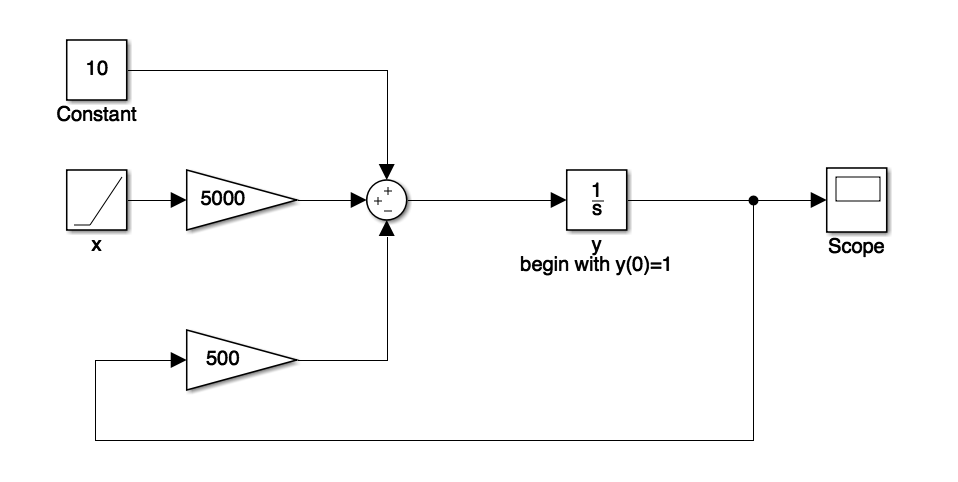
\includegraphics[width=0.7\linewidth]{A1_1_Schaltbild}
\caption{Simulink Schaltbild DGL1}
\label{fig:A1_1_Schaltbild}
\end{figure}

\subsection*{Iterationsgleichungen}
Im folgenden die Iterationsgleichungen der jeweiligen Verfahren.

\subsubsection*{Euler-Verfahren}
\begin{align}
x_{n+1} = x_{n}+h \\
y_{n+1} = y_{n}+h*f(x_{n},y_{n}) \\
y_{n+1} = y_{n}+h*(10-500y_{n}+5000x_{n})
\end{align}

\subsubsection*{Runge-Kutta-Verfahren 2.Ordnung}
\begin{align}
x_{n+1} = x_{n}+h \\
k_{1} = h*f(x_{n},y_{n}) \\
k_{1} = h*(10-500y_{n}+5000x_{n}) \\
k_{2} = h*f(x_{n} + \dfrac{h}{2},y_{n} + \dfrac{k_{1}}{2}) \\
k_{2} = h*(10-500*(y_{n} + \dfrac{k_{1}}{2})+5000*(x_{n} + \dfrac{h}{2})) \\
y_{n+1} = y_{n}+k_{2}
\end{align}

\end{document}
